%%%%%%%%%%%%%%%%%%%%%%%%%%%%%%%%%%%%%%%%%%%%%%%%%%%%%%%%%%%
%% Congratulations, you've made an excellent choice
%% of writing your Tampere University thesis using
%% the LaTeX system. This document attempts to be
%% as complete a template as possible to let you focus
%% on the most important part: the writing itself.
%% Thus the details regarding the visual appearance
%% and even structure have already been worked out
%% for you!
%%
%% I sincerely hope you will find this template useful
%% in completing your thesis project. I've tried to
%% add comments (followed by the % sign) to clarify
%% the structure and purpose of some of the commands.
%% Most of the magic happens in the file tauthesis.cls,
%% which you are more than welcome to take a look at.
%% Just refrain from editing it in the most crucial
%% versions of the thesis!
%%
%% I wish you and your thesis project the best of luck!
%% If this template causes you trouble along the way
%% or if you've any suggestions for improving it,
%% please contact me via email at
%%
%% ville.koljonen (at) tuni.fi.
%%
%% Yours,
%%
%% Ville Koljonen
%% 16th May 2019
%%
%% PS. This template or its associated class file don't
%% come with a warranty. The content is provided as is,
%% without even the implied promise of fitness to the
%% mentioned purpose. You, as the author of the thesis,
%% are responsible for the entire work, including the
%% provided material. No one else is liable to you for
%% any damage inflicted on you or your thesis, were it
%% caused by using this template or not.
%%%%%%%%%%%%%%%%%%%%%%%%%%%%%%%%%%%%%%%%%%%%%%%%%%%%%%%%%%%


%%%%% INSTRUCTIONS FOR COMPILING THE DOCUMENT %%%%%
%% Overleaf: just click Recompile.
%% Terminal:
%%  1. pdflatex main.tex
%%  2. makeindex -s main.ist -t main.glg -o main.gls main.glo
%%  3. biber main
%%  4. pdflatex main.tex
%%  5. pdflatex main.tex
%% Similar sequence of commands is also required
%% in LaTeX specific editors.
%%%%%%%%%%%%%%%%%%%%%%%%%%%%%%%%%%%%%%%%%%%%%%%%%%%

%%%%% PREAMBLE %%%%%

\nonstopmode
\documentclass{tauthesis}

% The glossaries package throws a warning:
% No language module detected for 'finnish'.
% You can safely ignore this. All other
% warnings should be taken care of!

%%%%% Your packages.
% Before adding packages, see if they can be found
% in tauthesis.cls already. If you're not sure that
% you need a certain package, don't include it in
% the document! This can dramatically reduce
% compilation time.

% Graphs
% \usepackage{pgfplots}
% \pgfplotsset{compat=1.15}

\usepackage{graphicx}

% Subfigures and wrapping text
\usepackage{subcaption}

% Mathematics packages

\usepackage{amsmath, amssymb, amsthm}
%\usepackage{bm}

%%%%% Your commands.

%%%%% Glossary information.

\loadglsentries[main]{tex/sanasto.tex}
\makeglossaries

%%%%% Citation information.

\addbibresource{tex/ilmari_references.bib}
\addbibresource{tex/niko_references.bib}

\hypersetup{hidelinks}

\begin{document}

%%%%% FRONT MATTER %%%%%

\frontmatter

%%%%% Thesis information and title page.

\title{Lämpöpumppujen kommunikaatiorajapinnat ja niiden hyödyntämismahdollisuudet}
\subtitle{Luonnos: versio 1}

% The author name.
\author{Ilmari Marttila, ja Niko Kangasniemi}

% The examiner information.
% If your work has multiple examiners, replace with
% \examiner[<label>]{<name> \\ <name>}
% where <label> is an appropriate (plural) label,
% e.g. Examiners or Tarkastajat, and <name>s are
% replaced by the examiner names, each on their
% separate line.
\examiner{Prof. Sami Repo}

% The finishing date of the thesis (YYYY-MM-DD).
\finishdate{2020}{01}{29}


\thesistype{Kandidaatintyö}

\facultyname{Informaatioteknologian ja viestinnän tiedekunta}
\programmename{Tieto- ja sähkötekniikan TkK-tutkinto-ohjelma - Sähkötekniikka}

\keywords%
    {}

\maketitle

%%%%% Abstracts and preface.

%\abstract{tex/tiivistelma.tex}

%\preface{tex/alkusanat.tex}{Tampereella}

%%%%% Table of contents.

\tableofcontents

%%%%% Lists of figures, tables, listings and terms.

\listoffigures
%\listoftables
%\lstlistoflistings


%\glossary

%%%%% MAIN MATTER %%%%%

\mainmatter
\chapter{Suunnitelma}
\section{Aiheen valinnan yhteydessä esitetty sisältöhahmotelma}
  Työssä voisin käsitellä esimerkiksi seuraavia aiheita.
  \begin{itemize}
    \item  Mikäli suuri määrä lämpöpumppuja olisi ohjattavissa keskitetysti, voidaan niitä käyttää virtuaalivoimalana tehonkulutushuippujen tasaamiseen. Monipuoliset rajapinnat voisivat mahdollistaa älykkään tehontarpeen priorisoinnin.
    \item Rajapintojen turvallisuus. Suojaamattomia yhteyksiä voidaan käyttää hyvän lisäksi myös pahaan.
    \item Listata ja vertailla olemassa olevien lämpöpumppujen sovelluskehittäjille tarjoamia rajapintoja.
    \item  Toimivatko lämmitysjärjestelmät nykyään luetettavasti myös ilman internet-yhteyttä? Entä tulevaisuudessa?
    \item Voisin esimerkiksi toteuttaa demotarkoitutksissa pienen käyttöliittymän johonkin valmiiseen lämpöpumppuun, mikäli sopiva ehdokas löytyy
  \end{itemize}
\section{Aiheanalyysi}

  Läpöpumppujen määrä kotitalouksissa on noussut runsaasti viimeisten vuosien aikana. Lämpöpumput nähdään ekologisena vaihtoehtona lämpöenergian tuottamiseen. Samaan aikaan sähköntuotanto on tietynlaisessa murroksessa, jossa keskitetystä tuotannosta siirrytään kohti hajautettua ja täten hankalammin ennustettavaa (ja säästä riippuvaa) sähöntuotantoa. Kun tuotannon vaihtelu lisääntyy, myös kulutuksen pitää olla joustavampaa.

  Selvitän työssäni mahdollisuuksia ja tapoja, joilla lämpöpumput voidaan ottaa mukaan tehontarpeen tasaukseen ja älykkään verkon toimintaan. Sitä ennen kuitenkin käydään läpi pumppujen sähkötekniikkaa ja sitä, miten pumput vaikuttavat sähköverkkoon. Teen myös katsauksen tapoihin ja teknologioihin, joilla pumppuja voidaan ohjata etänä. Olisi hienoa, jos saisin tehtyä jonkinlaisen pienen käytännön toteutuksen aiheesta, mutta en ole vielä löytänyt sopiavaa 

\section{sisältösuunnitelma}

\begin{enumerate}
  \item Johdanto
  \item Lämpöpumput sähkön käyttäjinä
    \begin{enumerate}
      \item Oikosulkumoottorit
      \item Taajuusmuuttajakäytöt
      \item Resistiivinen kuorma -- vastukset
    \end{enumerate}
  \item Rajapinnat -- eri abstraktiotasot
  \begin{enumerate}
    \item Smart Grid
    \item matalan tason kommunikointi
  \end{enumerate}
  \item lämpöpumppujen ohjauksella saavutettavat hyödyt
  \item käytännön toteutus tai simulointi
  \item yhteenveto
\end{enumerate}



\section{Aineistoja ja lähteitä}
  \begin{itemize}
    \item Perustietoa lämpöpumpuista. Luentokalvot kurssilta DEE-53100. \parencite{kummu}
    \item Yleiskästyksen luontia niistä ongelmista, mihin rajapintojen hyödyntämisellä voidaan vaikuttaa. \parencite[Luku 3]{rautiainen}
    \item Mielenkiintoista tietoa aiheesta. Johdattaa tutkimaan, mitä tarkoitetaan termillä \emph{SG-ready}. \parencite{ModelBasedFlexibilityAssessment}
    \item Käsitteleen myös muita kuorman tasaukseen liittyviä asioita \parencite{ShenJiangLi}
    \item Lisää aiheesta SG-ready \parencite{fischerTriebelSelinger}
    \item Modbus \parencite{sousaPortugal}
  \end{itemize}


%\chapter{Johdanto}
%\label{ch:johdanto}
%Lämpöpumppujen käyttö kiinteistöjen lämmitykseen kasvattaa suosiotaan. Vuoden 2000 jälkeen on Suomeen asennettu noin 700 000 lämpöpumppua\footnote{Alle \SI{26}{\kilo\watt}}\parencite{kummu}. Lämpöpumppujen kuluttama teho saattaa pienissä muuntopiireissä kasvaa hyvinkin merkittäväksi sen korvatessa vanhoja lämmitysmenetelmiä. Tämä aiheuttaa ongelmia sähkön siirrossa. Lämpöpumppuja, kuten monia muitakin sähköä käyttäviä laitteita, voidaan kuitenkin ohjata. On mahdollista toteuttaa paikallista kysyntäjoustoa ja ohjata lämpöpumppuja pientuotannon tuotantomäärien mukaan.

Lämpöpumppujen kasvanut suosio avaa myös uusia mahdollisuuksia. Suuria määriä lämpöpumppuja voidaan ohjata yhtenä ryhmänä. Ryhmää ohjaamalla voidaan toteuttaa kysyntäjoustoa jopa kansallisella tasolla ja vakauttaa säkövekon taajuutta ja jännitettä. Lämöpumppuryhmiä voidaan käyttää myös virtuaalivoimaloina ja niiden tehokapasiteettia voidaan myydä siitä maksaville\parencite{ShenJiangLi, fischerTriebelSelinger}.

Lämpöpumppuja on mahdollista siis käyttää osana älykästä sähköverkkoa. Lämpöpummpujen ohjaus voidaan mahdollistaa erilaisten rajapintojen kautta. Laitevalmistajien on tarjottava nämä rajapinnat. Rajapintoja voidaan toteuttaa monilla tavoilla ja valmiita teknisiä ratkaisuja on olemassa.


\chapter{Lämpöpumput sähkön käyttäjinä}
\label{ch:pumput_sahkon_kayttajina}
Tässä kappaleessa perehdytään lämpöpumpun toimintaperiaatteeseen ja siihen miten se käyttäytyy sähkön käyttäjänä. Lämpöpumpun vaikutukset sähköverkkoon riippuvat lämpöpumpun teknisistä ratkaisuista kuten tehon mitoituksesta ja moottorin syöttötavasta. Myös verkon ominaisuudet vaikuttavat pumpun käyttöön.

Lämpöpumppuja käytetään pääasiassa kiinteistöjen lämmitykseen ja viilennykseen. Muita kohteita ovat esimerkiksi teollisuus, jossa lämpöpumppujen avulla voidaan tuottaa prosessien tarpesiin lämpöä hyödyntämällä hukkalämpöä, tai kaukolämmöntuotanto.\parencite{Setala, katriVala} Lämpöpumppu saattaa olla kiinteistön ainoa lämmitysmuoto, tai se saattaa toimia toisten lämmitysjärjestelmien rinnalla. Lämpöpumpuilla voidaan korvata vanha järjestelmä, millä on vaikutusta kiinteistön lämmityksen aiheuttamaan sähkönkulutuksen luonteeseen. Esimerkiksi korvattaessa vanha öljy- tai puulämmitys lämpöpumpulla, sähkönkulutus kasvaa. Korvatessa suora sähkölämmitys lämpöpumpulla, muuttuu taas sähkön kulutuksen luonne. Lämpöpumppu käyttää saman lämmön tuottamiseen vähemmän sähköenergiaa, mutta huipputehot saattavat olla suurempia.

\section{Lämpöpumpun toimintaperiaate}
  Lämpöpumpun eli jäähdytyskoneen toimintaperiaate on käänteinen lämpövoimakoneelle. Lämpöpumppu siirtää lämpöenergiaa viileämmästä ympäristöstä lämpimämpään.\parencite{DincerRosen}

  Lämpöpumpun perusrakenne koostuu kompressorista, lauhduttimesta, paisuntaventtiilistä ja höyrystimestä, joiden välillä kiertää kylmäaine. Järjestelmä on kuvattu kuvassa \ref{fig:hptp}. Matalassa paineessa oleva kylmäaine höyrystyy viileämmässä tilassa sijaitsevassa höyrystimessä ja vastaanottaa lämpöenergiaa. Höyrystynyt kylmäaine johdetaan lauhduttimeen ja sen paine nostetaan kompressorin avulla korkeammaksi, jolloin sen lämpötila nousee. Korkeassa paineessa ja lämpötilassa oleva kylmäaine luovuttaa lämpöenergiaa lauhduttimen välityksellä lämpimään ympäristöön, jolloin osa siitä nesteytyy. Nesteytynyt kylmäaine virtaa paisuntaventtiilin kautta takaisin höyrystimeen. Paisuntaventtiilissä kylmäaineen paine ja täten myös lämpötila laskevat.\parencite{DincerRosen}

  Höyrystimessä lämpöenergiaa siirtyy kylmäaineeseen ympäristöstä. Lämmön kuljettaminen ympäristöstä höyrystimelle voidaan toteuttaa erilaisilla tavoilla. Suomessa yleisin tapa on käyttää ilmapuhallinta \parencite{sulpu}, joka puhaltaa ulkoilmaa höyrystimen lävitse ja jäähdyttää sitä. Tällöin kyseessä on ilmalämpöpumppu. Toinen yleinen vaihtoehto on käyttää maahan kaivettavaa tai kallioon porattavaa lämmönkeruuputkistoa. Tällaista lämpöpumppua kutsutaan maalämpöpumpuksi. Eri sovelluskohteissa käytetään myös lukuisia muitakin lämmönlähteitä kuten ilmanvaihdon poistoilmaa, viemärivettä, lauhdevettä tai vesistöä.\parencite{DincerRosen}

  Lauhduttimessa kylmäaineen luovuttama lämpöenergia siirretään sovelluskohteesta riippuen esimerkiksi käyttöveteen, lämmitysjärjestelmän vesikiertoon tai suoraan huoneilmaan. Teollisuudessa tuotettua energiaa voidaan käyttää esimerkiksi erilaisissa prosesseissa\parencite{Setala}. Sovelluskohde määrää lauhduttimelta vaadittavan lämpötilan. Järjestelmiä saatetaan kutsua erilaisilla nimillä riippuen siitä, mihin tuotettua energiaa käytetään. Mikäli tuotetulla energialla lämmitetään käyttövettä tai lämmitysjärjestelmän kiertovettä, kutsutaan laitetta Ilma--vesilämpöpumpuksi. \parencite{sulpu}

  Lämpöpumpun lämpökerroin, eli COP\footnote{Coefficient Of Performance} määritellään lämpöpumpun tuottaman lämpötehon ja sen kuluttaman sähkötehon suhteena
  \begin{equation}
      \textrm{COP} = \frac{\dot{Q}}{\dot{P}}
  \end{equation}
  Normaali lämpöpumppujen lämpökerroin vaihtelee välillä 2--5. Lämpökerroin ja sen vaihtelu riippuvat paljolti lämmön lähteestä: maalämpöpumpuilla on yleensä korkeampi lämpökerroin kuin ilmalämpöpumpuilla.\parencite{DincerRosen} Myös haluttu lauhduttimen lämpötila vaikkuttaa lämpökertoimeen. Mitä korkeampi lämpötila lauhduttimelle halutaan sen matalampi pumpun lämpökerroin on. \parencite[kuva 7.6]{DincerRosen}

  \begin{figure}
    \centering
    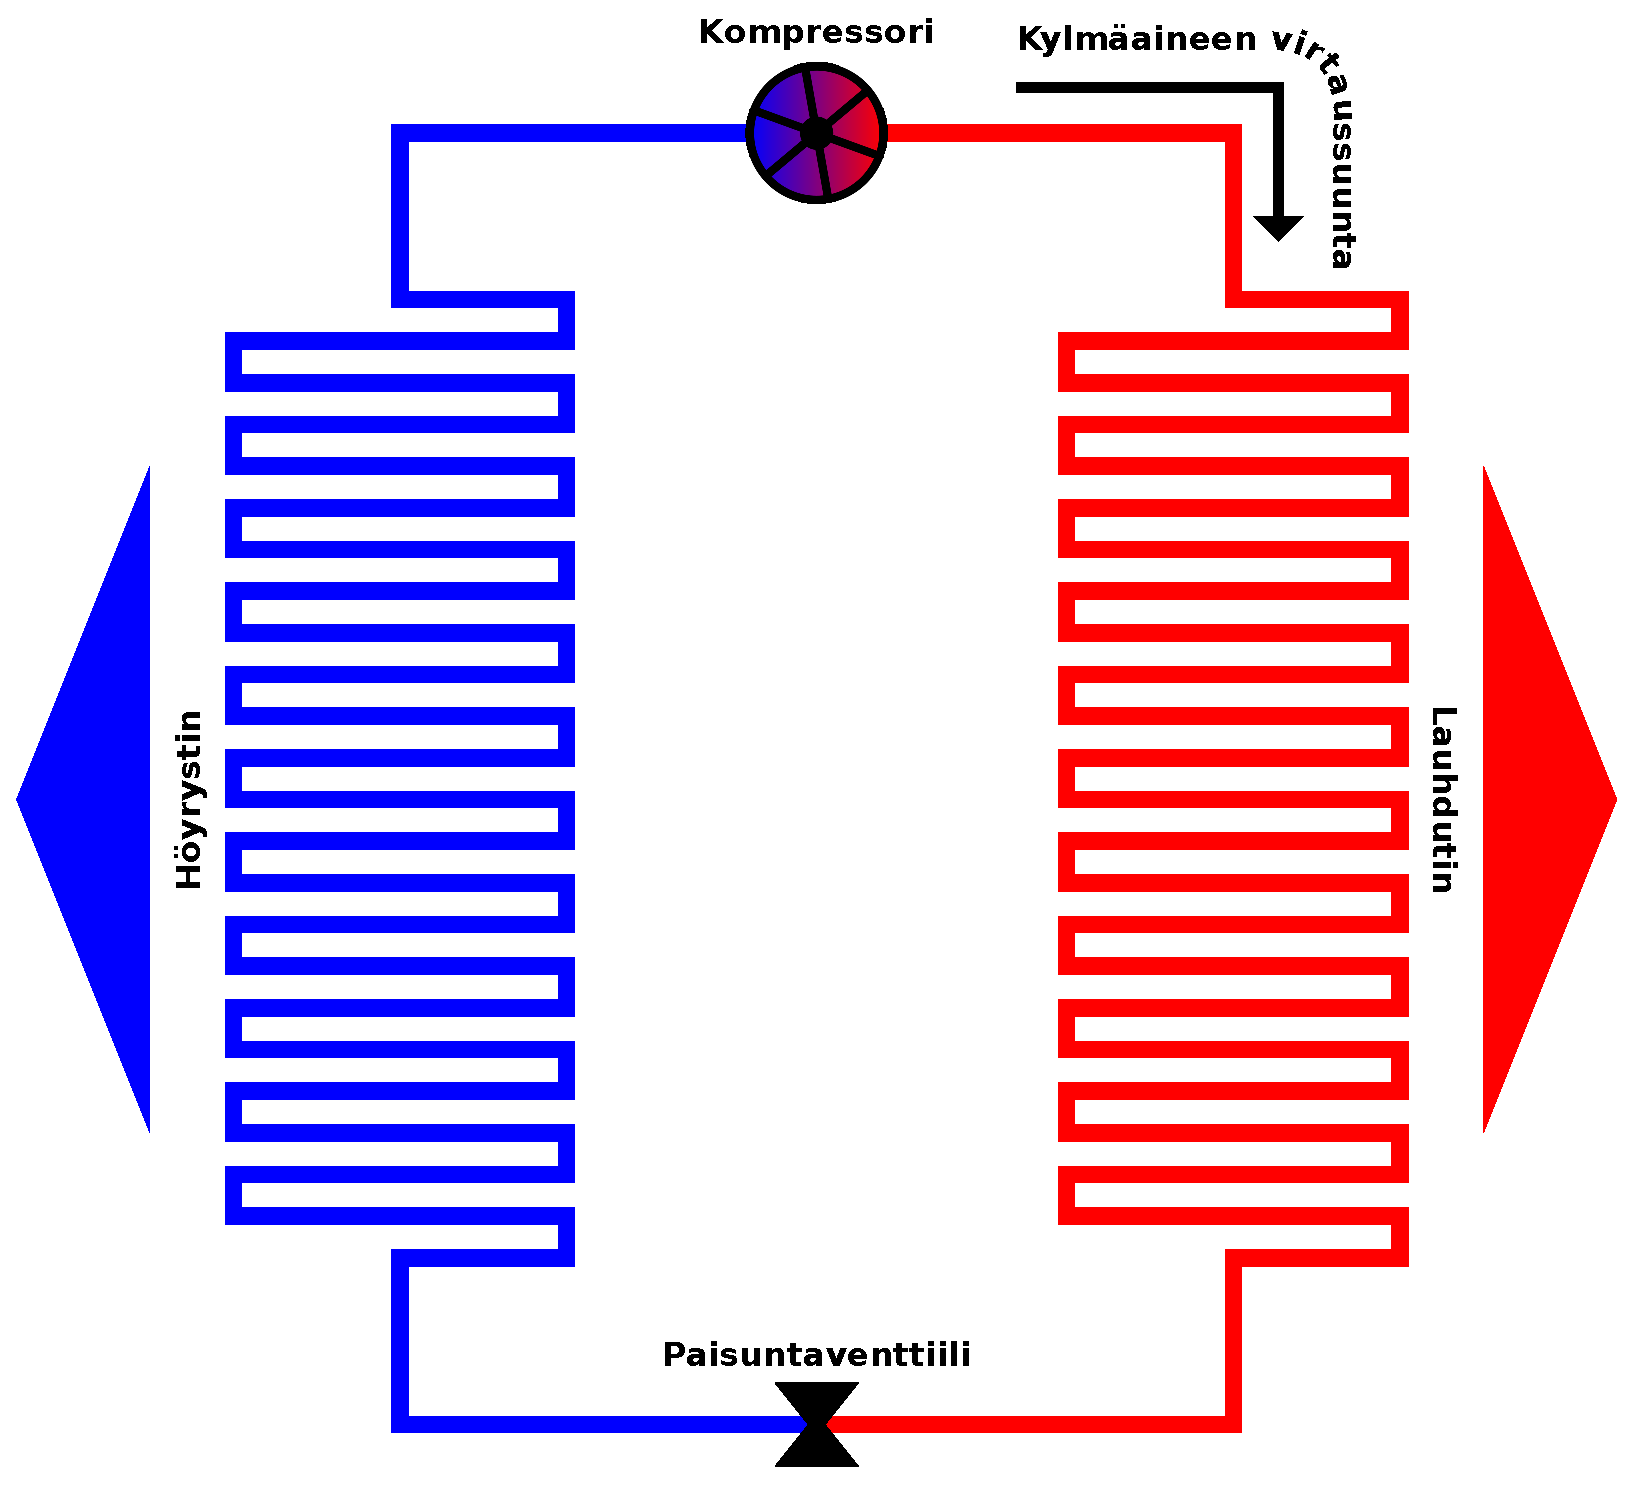
\includegraphics[width=0.5\textwidth]{figures/hp}
    \caption{Lämpöpumpun toimintaperiaate}
    \label{fig:hptp}
  \end{figure}

  Lämpöpumput käyttävät sähköenergiaa lämmön siirtämiseen viileämmästä lämpövarastosta lämpimämpään. Käytetystä sähköenergiasta valtaosa kuluu paineen tuottamiseen kompressorilla, mikä ylläpitää energiaa tuottavaa työkiertoa. Kompressorin lisäksi sähköä kuluu pienempiä määriä vaikkapa lämpöpumpun ohjaukseen, lämmitysjärjestelmän kiertovesipumpun käyttämiseen tai puhaltimen käyttämiseen. Mikäli lämpöpumpun teho on mitoitettu pienemmäksi kuin suurin vaadittu lämmitysteho\footnote{osatehomitoitus}, voidaan tehojen erotus tuottaa tarvittaessa lämpöpumpun yhteyteen asennettavilla sähkövastuksilla. Tällainen ratkaisu lisää huomattavasti järjestelmän sähkönkulutusta suurimman lämmitystarpeen aikana, jolloin sähköä käytetään muutenkin enemmän. Järjestelmän käyttäminen viilentämiseen taas lisää energian kulutusta, silloin kun sähkön käyttö on muuten todennäköisesti vähäisempää.

  Lämpöpumpuissa kompressorin pyörittämiseen käytetään sähkömoottoria. Vanhemmissa lämpöpumpuissa moottori on useimmiten verkkojännitteeseen kytketty oikosulkumoottori, joka voidaan tarvittaessa varustaa käynnistyksen ohjauksella eli pehmokäynnistimellä. Nykyaikaisemmassa ratkaisuissa oikosulkumoottoria käytetään taajuusmuuttajan avulla.

\section{Oikosulkumoottori}
  Yleisin tapa pyörittää lämpöpumpun kompressoria on käyttää suoraan verkkojännitteeseen kytkettyä oikosulkumoottoria. Kompressorin tehoa ei voida säädellä, vaan käydessään se tuottaa aina vakiotehon. Tällaisen lämpöpumpun tehoa säädetään kytkemällä kompressoria päälle ja pois. Kompressori kytkeytyy päälle, kun lämmitettävän kohteen, esimerkiksi lämminvesivaraajan tai sisäilman, lämpötila laskee tietyn rajan alapuolelle. Kun lämmitettävän kohteen lämpötila on noussut tarpeeksi, sammutetaan kompressori.

  Tärkeimmät kompressorin käyntijaksojen pituuteen vaikuttavat tekijät ovat lämmitettävän kohteen haluttu lämpötila ja lämpöenergian tarve, lämmönlähteen lämpötila ja kompressorin teho. Kotitalousköytössä kompressoreiden tehot ovat yleensä muutamia kilowatteja\footnote{etsi tarkempi tieto}.

  Mikäli oikosulkumoottorin käynnistysvirtaa ei mitenkään rajoiteta, on se tyypillisesti 6 -- 8 kertainen moottorin nimellisvirtaan nähden. Täten myös moottorin sähköverkosta käynnistyessään ottama teho on suuri.\parencite{pehmokaynnistinopas} Käynnistyksen jälkeen moottorin ottama virta ja teho laskevat kompressorin ottotehon määräämään arvoon.

  Oikosulkumoottorien suuret käynnistysvirrat näkyvät tehopiikkeinä myös sähköverkon puolella. Mikäli samassa muuntopiirissä on useampia lämpöpumppuja tai alhainen jännitejäykkyys, saattavat pumput aiheuttaa jännitetason vaihteluita. Alhaisen jännitejäykkyyden omaavissa verkoissa jo lämpöpumppujen normaalit käynnistykset saattavat aihetuttaa jännitetasonvaihteluita, jotka ilmenevät esimerkiksi välkyntänä\parencite{SFSEN50160}. Sähkökatkojen jälkeen kytkettäessä jännitettä takaisin, useat lämpöpumput saattavat käynnistyä samaan aikaan lämmittämään viilentyneitä lämmityskohteitaan. Tämä saattaa aiheuttaa lyhytaikaisen jännitteen aleneman. Mikäli jännitteenaleneman jälkeinen jäännösjännite on alle \SI{90}{\percent} järjestelmän nimellisjännitteestä, kutsutaan sitä jännitekuopaksi\parencite{SFSEN50160}.

  Oikosulkumoottoreiden käämityksistä johtuen ne ovat induktiivista kuormaa ja täten kuluttavat loistehoa. Mikäli moottoreiden kuluttamaa loistehoa ei kompensoida tuottamalla sitä paikallisesti, näyttäytyy lämpöpumppu sähköverkkoon induktiivisena kuormana. Induktiivisen kuorman kuluttama loisteho lisää häviöitä sähköverkossa ja loistehon kompensoinnin tarvertta verkkotasolla.\parencite{pakonen} \marginpar{onko kompensointia?}


\section{Oikosulkumoottori pehmokäynnistimellä}
  Lämpöpumpun käynnistyessään ottamaa virtapiikkiä voidaan pienentää tai se voidaan poistaa kokonaan pehmokäynnistimellä. Pehmokäynnistimen toiminta perustuu tyristoreihin, joilla säädellään moottorin kokemaa jännitettä. Alussa tyristorit johtavat vain hyvin pienen osan jännitteen jaksonajasta ja moottori alkaa tuottamaan momenttia. Vähitellen kasvatetaan tyristoreiden läpi päästettyä jännitteen osuutta, kunnes tyristorit ovat täysin johtavassa tilassa. Kun moottori on saavuttanut käyntinopeutensa, eivät tyristorit enää rajoita virtaa, ja ne voidaan esimerkiksi ohittaa kytkimellä tehohäviöiden pienentämiseksi.\parencite{pehmokaynnistinopas}

  Pehmokäynnistimen käyttö poistaa lämpöpumppujen käynnistysvirtapiikkien aiheuttaman ongelman. Pehmokäynnistimellä ei voida kuitenkaan järkevästi vaikuttaa moottorin käydessään ottamaan tehoon tai sen tuottamaan energiamäärään.

\section{Taajuusmuuttajakäytöt}
  Nykyaikainen ratkaisu lämpöpumpujen kompressorien käyttämiseen on taajuusmuuttaja. Taajuusmuuttaja koostuu tasasuuntaajasta ja ohjatusta vaihtosuuntaajasta, jolla saadaan tuotettua halutun suuruista ja taajuista vaihtojännitettä. Käynnistettäessä kompressoria aloitetaan moottorin syöttäminen matalataajuisella vaihtojännitteellä. Moottorin käyntinopeuden noustessa kohti haluttua arvoa, nostetaan samalla jännitteen taajuutta niin, että verkosta otettu teho pysyy suurin piirtein vakiona pyörimisnopeudesta riippumatta.

  Taajuusmuuttajan käytöllä saavutetaan useita hyötyjä. Käynnistysvirtapiikkien poistamisen lisäksi taajuusmuuttajalla voidaan myöskin säädellä kompressorin tuottamaa tehoa. Tehon säätäminen mahdollistaa pidemmät käyntijaksot ja tasaisemman tehonkulutuksen, mutta ei kuitenkaan vähennä lämpöpumpusta saatavaa maksimitehoa. Pienempien energiamäärien tuottaminen toteutetaan pienentämällä kompressorin käyntinopeutta, jolloin lämpöpumppua ei tarvitse käyttää useissa lyhyemmissä käyntijaksoissa.

  Verkon näkökulmasta taajuusmuuttaja näyttäytyy eri tavoilla riippuen siitä, miten siinä on totetutettu vaihtovirran tasasuuntaus. Perinteisissä ja halvemmissa taajuusmuuttajissa tasasuuntaus on toteutettu diodisillalla. Diodisilta aiheuttaa sisääntulevan virran säröytymistä ja sitä kautta myöskin jännitehäiriöitä verkkoon. Myöskään lämpöpumpun tehokertoimen säätäminen ei onnistu. Diodisiltaa parempi ratkaisu on verkkovaihtosuuntaaja, jonka ottama virta voidaan säätää lähes sinimuotoiseksi, jolloin virtasärön syntyminen voidaan ehkäistä. Verkkovaihtosuuntaajan tehokerrointa voidaan myöskin säätää, jolloin sitä voidaan käyttää loistehotasapainon ylläpitämiseen. Mikäli lämpöpumppua syöttävä taajuusmuuttaja on säädetty niin, että se näyttäytyy verkkoon lähes resistiivisenä kuormana se osaltaan vähentää verkon kuormitusta ja laskee jännitehäviöitä. Taajuusmuuttajan verkkoon aiheuttamat jännitehäiriöt riippuvat paljon taajuusmuuttajasta, sen laadusta ja koosta. \parencite{koskenjoki}

\section{Resistiivinen kuorma}
  Moottorikuormien lisäksi lämpöpumppujen yhteyteen asennetaan usein lämpövastuksia. Mikäli kyseessä on osatehomitoitettu lämpöpumppu, vastuksia käytetään suurimman energiatarpeen aikana, jolloin lämpöpumppu itsessään ei kykene tuottamaan kaikkea tarvittavaa energiaa. Lämpövastuksia käytetään myöskin höyrystimeen kertyneen jään ja huurteen poistoon.

  Lämpöpumpuissa kuluu sähköä myös muihin tarkoituksiin kuin suoraan energiantuotantoon. Automatiikan, ohjauksen ja sisä- ja ulkoyksiköiden puhaltimien kuluttama energia on kuitenkin vähäistä verrattuna muuhun energiankulutukseen


%\chapter{Yhteenveto}
%\label{ch:yhteenveto}
%Lämpöpumppujen ja aurinkosähköjärjestelmien merkitys sähköverkossa kasvaa niiden suosion kasvaessa. Lämpöpumput korvaavat muita lämmitys- ja viilennysmuotoja ja aurinkosähköjärjestelmillä haetaan kotitalouksissa omavaraisuutta ja ylipäätään säästöjä sähkölaskussa.

Aurinkosähköjärjestelmien määrän kasvu lisää sähköverkon tuotannon ailahtelevuutta ja säätövoiman tarvetta, sillä tuotanto vaihtelee tunneittain. Tuotantoa voidaan ennustaa sääennusteen pohjalta, mutta yksittäiset pilvet voivat aiheuttaa alueellisesti nopeitakin tehovaihteluita. Lisäksi huipputeho sijoittuu päiväsaikaan, joten ihmisten palatessa töistä ja kulutuksen kasvaessa tuotannon laskiessa samanaikaisesti säätötehon tarve kasvaa entisestään.

Lämpöpumppujen lisääntyminen ja esimerkiksi suorasta sähkölämmityksestä eroava käyttäytyminen vaikuttavat sähköverkkoon. Lämpöpumppujen tekniikka kehittyy ja nykyisin kotitalouskäyttöön myytävissä pumpuissa on yleensä suoraan verkkoon kytketyn oikosulkumoottorin tilalla taajuusmuuttajakäyttöinen oikosulkumoottori. Tämä kehitys myös osaltaan määrittelee miten verkkoon liitettyjen lämpöpumppujen määrän kasvu vaikuttaa sähköverkkoon. Ilman taajuusmuuttajaa tai pehmokäynnistintä verkkoon kytketyt lämpöpumput ottavat käynnistyessään verkosta suuria hetkellisiä tehoja, mikä saattaa jännitejäykkyydeltään huonossa verkossa aiheuttaa hetkellisiä jännitteenalenemia. Lämpöpumpun ollessa taajuusmuuttajakäyttöinen, ei se aiheuta edellä mainittuja tehonkulutuksen piikkejä. Kuitenkin mikäli lämpöpumpulla korvataan jokin muu lämmitysmuoto, kuin suora sähkölämmitys, kasvattaa se kulutuspaikan sähköenergian kulutusta. Mikäli muuntopiirissä moni talous vaihtaa lämmitysmuodokseen lämpöpumpun, saattaa se aiheuttaa tarpeen sähköverkon jännitejäykkyyden parantamiselle.

Järjestelmien tuomia haasteita voidaan ratkaista ja löytää uusia järjestelmiä hyödyntäviä sovelluksia, kun kommunikaatio niiden kanssa mahdollista. Kommunikointi mahdollistetaan standardoiduilla kommunikaatiorajapinnoilla, joiden kautta järjestelmiä voidaan ohjata. Tällöin ne voidaan kytkeä esimerkiksi kiinteistöautomaatioon tai muuhun ulkoiseen ohjaukseen. Valmistajien suljetut pilvipalvelut muodostavat myös erään rajapinnan kommunikaatiolle, joihin pääsy on usein vain valmistajalla ja järjestelmän omistajalla.

Yksi suosituimmista järjestelmien ohjauksen mahdollistavista tekniikoista on Modbus. Modbus-standardi määrittelee fyysisen tason rajapinnat mahdollistaen ohjauksen joko sarja- tai Ethernet-liitäntää käyttäen, mikä mahdollistaa protokollan käyttämisen paikallisesti tai internetin yli toimivien etäyhteyksien välityksellä. Modbus-standardin määritellessä kommunikointia vain hyvin matalalla tasolla on sitä helppo soveltaa erilaisiin sovelluksiin ja sen päälle voidaan rakentaa korkeamman tason viestintä- ja ohjausprotokollia. Modbusin päälle voidaan myöskin toteuttaa yksittäisen laitteen ohjaukseen ja monitorointiin tarvittavat sovellukset tai liittäminen kotiautomaatioon osaksi älykästä kotia.

Aurinkosähköjärjestelmien ja energiavarastojen osalta työssä tarkasteltiin muutamia eri rajapintoja, joista tärkein on SunSpec Modbus. Se pohjautuu Modbus-standardiin, ja sen avulla voidaan ohjata energiavarastojen ja aurinkosähköinverttereiden toimintaa, esimerkiksi rajoittaa tehoa tai säätää loistehontuotantoa. Suurin käyttö tällä rajapinnalla on paikallisessa automaatiossa, esimerkiksi tuotantotietojen käyttö kuormanohjaukseen.

Lämpöpumppujen kohdalla korkeamman tason rajapintoja kuten SG-Ready-ohjausrajapintaa tai Saksalaista EVU-Sperre-ohjausrajapintaa käyttävät sovellukset taas keskittyvät yhden lämpöpumpun sijasta useamman pumpun muodostamaan pooliin. Lämpöpumppupoolin ohjaamista voidaan käyttää erilaisiin sovelluksiin kuten huipputehon rajoittamiseen verkossa tai sähköntuotannon ja -kulutuksen tasapainottamiseen. Aggregaattorin hallinnoimaa lämpöpumppupoolia voidaan käyttää esimerkiksi kysyntäjouston tehokkaaseen toteuttamiseen. Aggregaattorille lämpöpumppupoolin ohjaaminen taas on pääasiallista liiketoimintaa, jolla se osallistuu sähkömarkkinoille.

Työssä tarkasteltiin kuutta eri sidosryhmää, joista Fingrid on sidoksissa vain aurinkosähköjärjestelmiin. Muut sidosryhmät hyödyntävät eri kommunikaatiorajapintoja eri tarkoituksiin, joista osalle niiden käyttö voi olla myös yrityksen ydinliiketoimintaa.

Rajapinnat mahdollistavat useita sovelluksia, mutta kaikki käsitellyt sovellukset eivät vielä ole yleistyneet Suomessa. Etämonitorointi ja -hallinta on ollut jo pidempään käytössä pilvipalveluiden muodossa, ja kiinteistöautomaatio yleistyy kotitalouksissa energiansäästötarkoituksessa.

Kysyntäjousto on vasta yleistymässä Suomessa, sillä aggregaattoreita ei Suomessa oikeastaan ole. Itsenäisen aggregaattorin laajennettu pilotti käynnistyi 21.7.2020, ja siinä testataan aiemmin kokeiltujen ratkaisujen skaalautuvuutta. Fingrid on ajamassa tätä kaikille säätösähkömarkkinoille avointa pilottia eteenpäin.

Teollisuuslaitosten tarvitsemia loistehon kompensaattoreita voidaan tulevaisuudessa korvata aurinkosähköjärjestelmillä, sillä suuritehoiset invertterit voivat tuottaa nimellistehollaan myös loistehoa ympäri vuorokauden. Tällöin kalliiden loistehon kompensaattoreiden takaisinmaksuaikaa voidaan pienentää, kun sitä voidaan hyödyntää myös sähköntuotantoon.

Kommunikaatiorajapintojen hyödyntäminen vaatii vahvaa standardointia, jotta järjestelmät olisivat valmistajasta riippumattomia. Järjestelmien fyysisten rajapintojen osalta tämä alkaa olla jo hyvällä mallilla, mutta niiden hyödyntäminen vaatii vielä kehittämistä. Vielä on kysymysmerkkinä, miten esimerkiksi Suomessa aggregaattori voi ohjata poolina akullisia aurinkosähköjärjestelmiä, tai mitä rajapintaa se käyttäisi virtuaalivoimalaitoksen kautta yksittäisten lämpöpumppujen ohjaamiseen.


\printbibliography[heading=bibintoc]

%%%%% Appendices.

%\begin{appendices}

%\chapter{Esimerkkiliite}
%\label{ch:liite}
%Tämä on liite


%\end{appendices}

\end{document}
